\chapter{Модели привилегированного обучения и дистилляции}

Раздел посвящен методам понижения сложности аппроксимирующих моделей. Предлагается вероятностное обоснование методов дистилляции и привилегированного обучения.
В данной главе рассматривается вероятностный подход к решению задачи дистилляции модели и задачи привилегированного обучения.
Проанализирована задача обучения модели ученика с помощью модели учителя. Исследован метод дистилляции и привилегированного обучения.
Предложено вероятностное обоснование дистилляции.

Приведены общие выводы для произвольной параметрической функции с наперед заданной структурой.
Приводится теоретическое обоснование для частных случаев: линейной и логистической регрессии.
Подход обобщается на случай, когда привилегированная информация доступна не для всех объектов из обучающей выборки.
В рамках вероятностного подхода предлагается анализ и обобщение функции ошибки~\cite{Hinton2015, Lopez2016}.
Рассматриваются частные задачи классификации и регрессии~\cite{Ivakhnenko1994}.

В главе введены вероятностные предположения, описывающие дистилляцию моделей.
В рамках данных вероятностных предположений анализируются модели для задачи классификации и регрессии.
Результат анализа сформулирован в виде теорем~\ref{theorem:st:dist}~и~\ref{theorem:st:reg}.
Теорема~\ref{theorem:st:reg} показала, что обучение линейной регрессии с учителем эквивалентно замене обучающей выборки и вероятностных предположений о распределении истинных ответов.
Для задачи классификации ответы учителя дают дополнительную информацию в виде распределения классов для каждого объекта из обучающей выборки.
Данная информация не может быть представлена в виде классической задачи классификации. Требуется ввести распределение, которое представлено в теореме~\ref{theorem:st:dist}.

В вычислительном эксперименте анализируются методы как использующие, так и не использующие модель учителя при обучении модели ученика. Проведен анализ ответов модели ученика с использованием модели учителя и без нее.

Анализируются рассмотренные модели на синтетических выборках и реальных данных. В качестве реальных данных рассматриваются выборки FashionMNIST~\cite{fashionmnist} и Twitter Sentiment Analysis~\cite{twiter2013}. Выборка FashionMNIST~\cite{fashionmnist} является реальной выборкой для задачи классификации изображений, а выборка для Twitter Sentiment. Выборка FashionMNIST использовалась вместо выборки MNIST, так как последняя имеет приемлемое качество аппроксимации даже для линейного классификатора. Analysis~\cite{twiter2013}~--- задачи классификации текстов. Вычислительный эксперимент использует модели разной сложности: линейная модель, полносвязная нейронная сеть, сверточная нейронная сеть~\cite{LeCun1989}, модель Bi-LSTM~\cite{Schmidhuber1997} и модель BERT~\cite{Devlin2018}.

Основным результатом данной главы является вероятностная интерпретация задачи дистилляции. Рассмотрен частный случай, когда признаковые описания модели учителя и ученика совпадают.

\section{Обобщенная вероятностная постановка задачи дистилляции}
Задано распределение целевой переменной~$p\bigr(\mathbf{y}_i|\mathbf{x}_i, \mathbf{g}\bigr)$.
Для поиска~$\hat{\mathbf{g}}$ воспользуемся методом максимального правдоподобия. В качестве~$\hat{\mathbf{g}}$ выбирается функция, которая максимизирует правдоподобие модели:
\begin{gather}
\label{eq:st:7}
\begin{aligned}
\hat{\mathbf{g}} = \arg\max_{\mathbf{g}\in \mathfrak{G}} \prod_{i=1}^{N}p\bigr(\mathbf{y}_{i}|\mathbf{x}_i, \mathbf{g}\bigr),
\end{aligned}
\end{gather}
где множество~$\mathfrak{G}$ задается~в~\eqref{eq:st:G}.
\subsection{Подход дистилляции модели учителя в модель ученика}
Рассмотрим вероятностную постановку, в которой выполнены ограничения:
\begin{enumerate}[1)]
	\item задано распределение целевой переменной~$p\bigr(\mathbf{y}_i|\mathbf{x}_i, \mathbf{g}\bigr)$;
	\item задано совместное распределение целевой переменной и ответов модели учителя~$p\bigr(\mathbf{y}_i, \mathbf{s}_i|\mathbf{x}_i, \mathbf{g}\bigr)$;
	\item для всех $\omega \in \bm{\Omega}^*$ элементы $\mathbf{y}(\omega)$ и $\mathbf{s}(\omega)$ являются зависимыми величинами, так как ответы учителя должны коррелировать с истинными ответами;
	\item если $|\bm{\Omega}^*|=0$, то решение должно соответствовать решению~\eqref{eq:st:7}.
\end{enumerate}

Рассмотрим совместное правдоподобие истинных меток и меток учителя:
\begin{gather}
\label{eq:st:8}
\begin{aligned}
p\bigr(\mathbf{Y}, \mathbf{S}|\mathbf{X}, \mathbf{g}, \mathcal{I}\bigr)=\prod_{i\not\in \mathcal{I}}p\bigr(\mathbf{y}_i|\mathbf{x}_i, \mathbf{g}\bigr)\prod_{i\in \mathcal{I}}p\bigr(\mathbf{y}_i, \mathbf{s}_i|\mathbf{x}_i, \mathbf{g}\bigr).
\end{aligned}
\end{gather}
Перепишем~$p\bigr(\mathbf{y}_i, \mathbf{s}_i|\mathbf{x}_i, \mathbf{g}\bigr)$ по формуле условной вероятности:
\begin{gather}
\label{eq:st:bernuli}
\begin{aligned}
p\bigr(\mathbf{y}_i, \mathbf{s}_i|\mathbf{x}_i, \mathbf{g}\bigr) = p\bigr(\mathbf{y}_i|\mathbf{x}_i, \mathbf{g}\bigr)p\bigr(\mathbf{s}_i|\mathbf{y}_i, \mathbf{x}_i, \mathbf{g}\bigr).
\end{aligned}
\end{gather}
Подставляя выражения~\eqref{eq:st:bernuli} в~\eqref{eq:st:8}, получим
\begin{gather}
\label{eq:st:9}
\begin{aligned}
p\bigr(\mathbf{Y}, \mathbf{S}|\mathbf{X}, \mathbf{g}, \mathcal{I}\bigr)=\prod_{i\not\in \mathcal{I}}p\bigr(\mathbf{y}_i|\mathbf{x}_i, \mathbf{g}\bigr)\prod_{i\in \mathcal{I}}p\bigr(\mathbf{y}_i|\mathbf{x}_i, \mathbf{g}\bigr)\prod_{i\in \mathcal{I}}p\bigr(\mathbf{s}_i|\mathbf{y}_i, \mathbf{x}_i, \mathbf{g}\bigr).
\end{aligned}
\end{gather}
Заметим, что~$\mathbf{y}_i$ и~$\mathbf{s}_i$ зависимы только через переменную~$\mathbf{x}_i$, тогда~$p\bigr(\mathbf{s}_i|\mathbf{y}_i, \mathbf{x}_i, \mathbf{g}\bigr)=p\bigr(\mathbf{s}_i|\mathbf{x}_i, \mathbf{g}\bigr)$. Получаем совместное правдоподобие
\begin{gather}
\label{eq:st:10}
\begin{aligned}
p\bigr(\mathbf{Y}, \mathbf{S}|\mathbf{X}, \mathbf{g}, \mathcal{I}\bigr)=\prod_{i\not\in \mathcal{I}}p\bigr(\mathbf{y}_i|\mathbf{x}_i, \mathbf{g}\bigr)\prod_{i\in \mathcal{I}}p\bigr(\mathbf{y}_i|\mathbf{x}_i, \mathbf{g}\bigr)\prod_{i\in \mathcal{I}}p\bigr(\mathbf{s}_i|\mathbf{x}_i, \mathbf{g}\bigr).
\end{aligned}
\end{gather}
Используя~\eqref{eq:st:10}, получаем оптимизационную задачу для поиска~$\hat{\mathbf{g}}$
\begin{gather}
\label{eq:st:11}
\begin{aligned}
\hat{\mathbf{g}} = \arg\max_{\mathbf{g}\in \mathcal{G}} \prod_{i\not\in \mathcal{I}}p\bigr(\mathbf{y}_i|\mathbf{x}_i, \mathbf{g}\bigr)\prod_{i\in \mathcal{I}}p\bigr(\mathbf{y}_i|\mathbf{x}_i, \mathbf{g}\bigr)\prod_{i\in \mathcal{I}}p\bigr(\mathbf{s}_i|\mathbf{x}_i, \mathbf{g}\bigr).
\end{aligned}
\end{gather}
Для удобства минимизируется логарифм выражения. Тогда из~\eqref{eq:st:11} получаем, что
\begin{gather}
\label{eq:st:12}
\begin{aligned}
\hat{\mathbf{g}} = \arg\max_{\mathbf{g}\in \mathcal{G}} \sum_{i\not\in \mathcal{I}}\log p\bigr(\mathbf{y}_i|\mathbf{x}_i, \mathbf{g}\bigr) + \left(1-\lambda\right)\sum_{i\in \mathcal{I}}\log p\bigr(\mathbf{y}_i|\mathbf{x}_i, \mathbf{g}\bigr) + \lambda\sum_{i\in \mathcal{I}}\log p\bigr(\mathbf{s}_i|\mathbf{x}_i, \mathbf{g}\bigr),
\end{aligned}
\end{gather}
где параметр~$\lambda \in [0,1]$ введен для взвешивания ошибок на истинных ответах и ошибок ответов учителя.

На рис.~\ref{fg:st:plate} показан вид вероятностной модели в графовой нотации для произвольной функции~$\mathbf{g}$.

\begin{figure}[h!]\center
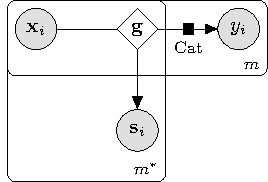
\includegraphics[width=0.35\textwidth]{results/privlearn/general_model}
\caption{Вероятностная модель в графовой нотации.}
\label{fg:st:plate}
\end{figure}

Для каждой реализации~$\mathbf{g}$ соответствующий блок требует уточнения. На рис.~\ref{fg:ex:synt:plate} показана более подробная реализация в случае, когда~$\mathbf{g}$~--- линейная модель.

\paragraph{Классификация.} Для задачи многоклассовой классификации рассматриваются вероятностные 
{\sl{п\,р\,е\,д\,п\,о\,л\,о\,ж\,е\,н\,и\,я:}}
\begin{enumerate}[1)]
\label{st:class:1}
	\item \emph{рассматривается функция учителя} $\mathbf{f}\in\mathfrak{F}_{\text{cl}}^{*}$~\emph{\eqref{eq:F:set:cl:priv};}
	\item \emph{рассматривается функция ученика}   $\mathbf{g}\in\mathfrak{G}_{\text{cl}}$~\emph{\eqref{eq:G:set:cl};}
	\item \emph{для истинных меток рассматривается категориальное распределение}~$p\bigr(y|\mathbf{x}, \mathbf{g}\bigr) = \text{Cat}\bigr(\mathbf{g}\bigr(\mathbf{x}\bigr)\bigr)$, \emph{где $\mathbf{g}\bigr(\mathbf{x}\bigr)$ задает вероятность каждого класса;}
	\item \emph{для меток учителя введем плотность распределения}
\begin{gather}
\label{reg:dist}
\begin{aligned}
	p\bigr(\mathbf{s}|\mathbf{x}, \mathbf{g}\bigr) = C\prod_{k=1}^{K}g_k\bigr(\mathbf{x}\bigr)^{s^k},
\end{aligned}
\end{gather}
\emph{где~$g^k$~--- вероятность класса~$k$, которую предсказывает модель ученика, а~$s^k$~--- вероятность класса~$k$, которую предсказывает модель учителя.}
\end{enumerate}
\begin{theorem}
\label{theorem:st:dist}
Пусть вероятность каждого класса отделима от нуля и единицы, т.е. для всех~$k$ выполняется условие
\[1 > 1- \varepsilon > g_k\bigr(\mathbf{x}\bigr) > \varepsilon > 0.
\]

Тогда при
\begin{gather}
C=\left(-1\right)^{K}\frac{K^{K/2}}{2^{K(K-1)/2}}\prod_{k=1}^{K}g_k\bigr(\mathbf{x}\bigr)\log g_k\bigr(\mathbf{x}\bigr)
\end{gather}
функция $p\bigr(\mathbf{s}|\mathbf{x}, \mathbf{g}\bigr)$, определенная в~\eqref{reg:dist}, является плотностью распределения.
\end{theorem}
\begin{proof}
	Во-первых, покажем, что для произвольного вектора ответов $\mathbf{s} \in \mathcal{S}_K$ выполняется $p\bigr(\mathbf{s}|\mathbf{x}, \mathbf{g}\bigr) \geq 0$. Заметим, что для всех~$k$ выполняется
	\[\log g_k\bigr(\mathbf{x}\bigr) < 0,\] тогда
\begin{gather}
\begin{aligned}
	C=\underbrace{\frac{K^{K/2}}{2^{K(K-1)/2}}}_{>0}\prod_{k=1}^{K}\underbrace{g_k\bigr(\mathbf{x}\bigr)}_{>\varepsilon}\underbrace{\left(-\log g_k\bigr(\mathbf{x}\bigr)\right)}_{>0} > 0.
\end{aligned}
\end{gather}
Так как~$g_k\bigr(\mathbf{x}\bigr) >0$ и~$C>0$, получаем, что $p\bigr(\mathbf{s}|\mathbf{x}, \mathbf{g}\bigr) \geq 0$.
	Во-вторых, покажем, что интеграл по всему пространству ответов~$\mathcal{S}_K$ является конечным:
	\begin{gather}
	\label{theorem:st:dist:eq:1}
	\begin{aligned}
		\int\limits_{\mathcal{S}_K}&p\bigr(\mathbf{s}|\mathbf{x}, \mathbf{g}\bigr)ds = \int\limits_{\mathcal{S}_K}\prod_{k=1}^{K}g_k\bigr(\mathbf{x}\bigr)^{s^k}ds = \prod_{k=1}^{K}\int\limits_{\mathcal{S}_K}g_k\bigr(\mathbf{x}\bigr)^{s^k}ds =\\ 
		& = \prod_{k=1}^{K}\int\limits_{0}^{1}\frac{r^{K-1}\sqrt{K}}{\left(K-1\right)!\sqrt{2^{K-1}}}g_k\bigr(\mathbf{x}\bigr)^{r}dr = \prod_{k=1}^{K}\underbrace{\frac{\sqrt{K}}{\left(K-1\right)!\sqrt{2^{K-1}}}}_{D}\int\limits_{0}^{1}r^{K-1}g_k\bigr(\mathbf{x}\bigr)^{r}dr =\\
		& = D^K\prod_{k=1}^{K} \int\limits_{0}^{1}r^{K-1}\exp\bigr(r\log g_k\bigr(\mathbf{x}\bigr)\bigr)dr =\\
		& = \left(-D\right)^K\prod_{k=1}^{K}\log g_k\bigr(\mathbf{x}\bigr)\left(\Gamma\bigr(K\bigr) - \Gamma\bigr(K, -\log g_k\bigr(\mathbf{x}\bigr)\bigr)\right) =\\
		& = \left(-D\right)^K\left(K-1\right)!^K\prod_{k=1}^{K}\log g_k\bigr(\mathbf{x}\bigr)\left(1 -g_k\bigr(\mathbf{x}\bigr) \exp_{K-1}\bigr(-\log g_k\bigr(\mathbf{x}\bigr)\bigr)+g_k\bigr(\mathbf{x}\bigr)\right) =\\
		& = \frac{\left(-\sqrt{K}\right)^K}{2^{K(K-1)/2}}\prod_{k=1}^{K}\log g_k\bigr(\mathbf{x}\bigr)\left(1 -g_k\bigr(\mathbf{x}\bigr) \exp_{K-1}\bigr(-\log g_k\bigr(\mathbf{x}\bigr)\bigr)+g_k\bigr(\mathbf{x}\bigr)\right) < \infty,
	\end{aligned}
	\end{gather}
где~$\Gamma\bigr(K\bigr)$ является гамма-функцией, $\Gamma\bigr(K, -\log g_k\bigr(\mathbf{x}\bigr)\bigr)$ является неполной гамма функцией, $\exp_{r}\bigr(x\bigr)$ является суммой Тейлора из первых~$r$ слагаемых. В рамках приближенных расчетов считается, что $\exp_{r}\bigr(x\bigr)\approx\exp\bigr(x\bigr),$ тогда с учетом~\eqref{theorem:st:dist:eq:1} получаем
	\begin{gather}
	\label{theorem:st:dist:eq:2}
	\begin{aligned}
		C\bigr(\mathbf{g}, \mathbf{x}\bigr) = \int\limits_{\mathcal{S}_K}p\bigr(\mathbf{s}|\mathbf{x}, \mathbf{g}\bigr)ds \approx \left(-1\right)^{K}\frac{K^{K/2}}{2^{K(K-1)/2}}\prod_{k=1}^{K}g_k\bigr(\mathbf{x}\bigr)\log g_k\bigr(\mathbf{x}\bigr).
	\end{aligned}
	\end{gather}
Полученное выражение~\eqref{theorem:st:dist:eq:2} заканчивает доказательство теоремы~1.
\end{proof}

Из теоремы~\ref{theorem:st:dist} следует, что плотность, введенная для меток учителя, является плотностью распределения. Поэтому можно воспользоваться выражением~\eqref{eq:st:12}.
Используя предположения 1--4 и подставляя в~\eqref{eq:st:12}, получаем  оптимизационную задачу:
\begin{gather}
\label{eq:st:class:1}
\begin{aligned}
\hat{\mathbf{g}} = \arg\max_{\mathbf{g}\in \mathcal{G}} & \sum_{i\not\in \mathcal{I}}\sum_{k=1}^{K}y_i^k\log g_k\bigr(\mathbf{x}_i\bigr)\bigr|_{T=1} +\\
&+ \left(1-\lambda\right)\sum_{i\in \mathcal{I}}\sum_{k=1}^{K}y_i^k\log g_k\bigr(\mathbf{x}_i\bigr)\bigr|_{T=1} + \lambda\sum_{i\in \mathcal{I}}\sum_{k=1}^{K}s_{i,k}\log g_k\bigr(\mathbf{x}_i\bigr)\bigr|_{T=T_0} +\\
&+ \lambda \sum_{i\in \mathcal{I}}\sum_{k=1}^{K}\left(\log g_k\bigr(\mathbf{x}_i\bigr)\bigr|_{T=T_0} + \log\log\frac{1}{g_k\bigr(\mathbf{x}_i\bigr)}\bigr|_{T=T_0}\right).
\end{aligned}
\end{gather}

Проанализировав выражение~\eqref{eq:st:class:1}, получаем, что первые три слагаемых совпадают со слагаемыми в выражении~\eqref{eq:hinton:1} при~$\mathcal{I} = \{1, \ldots, m\}$ и $\lambda=\frac{1}{2}$, а четвертое слагаемое является некоторым регуляризатором, который получен из вида распределения. Анализируя первые три слагаемых в выражении~\eqref{eq:st:class:1} при~$T_0 = 1$, получаем сумму кросс-энтропий между двумя распределениями для каждого объекта:
\begin{enumerate}[1)]
	\item первое распределение~--- это выпуклая комбинация с весами~$1-\lambda$ и $\lambda$ распределения, задаваемого метками объектов~$\text{Cat}\bigr(\mathbf{y}\bigr)$, и распределения, задаваемого моделью учителя~$\text{Cat}\bigr(\mathbf{s}\bigr)$;
	\item второе распределение~--- это распределение, задаваемое моделью ученика~$\text{Cat}\bigr(\mathbf{g}\bigr(\mathbf{x}\bigr)\bigr)$.
\end{enumerate}

Следовательно, модель ученика восстанавливает плотность не исходных меток, а новую плотность, которая является выпуклой комбинацией плотности исходных меток и меток учителя.

\paragraph{Регрессия.} Для задачи регрессии рассматриваются вероятностные \emph{п\,р\,е\,д\,п\,о\,л\,о\,ж\,е\,н\,и\,я:}

\begin{enumerate}[1)]
	\item \emph{рассматривается функция учителя~$\mathbf{f}\in\mathfrak{F}_{\text{rg}}^{*}$,
	%\begin{gather}
	%\label{eq:F:set:priv}
	%\begin{aligned}
	\[
	\mathfrak{F}_{\text{rg}}^* = \left\{\mathbf{f}| \mathbf{f} = \mathbf{v}^*\bigr(\mathbf{x}^*\bigr), \quad \mathbf{v}^*: \mathbb{R}^{n^*} \to \mathbb{R} \right\},
	\]
	%\end{aligned}
	%\end{gather}
	где~$\mathbf{v}^*$~--- дифференцируемая параметрическая функция;}
	\item \emph{рассматривается функция ученика~$\mathbf{g}\in\mathfrak{G}_{\text{rg}}$,
    %\begin{gather}
    %\label{eq:G:set:rg}
    \[
    \mathfrak{G}_{\text{rg}} = \left\{\mathbf{g}| \mathbf{g} = \mathbf{z}\bigr(\mathbf{x}\bigr), \quad \mathbf{z}: \mathbb{R}^n \to \mathbb{R}^K \right\},
    \]
    %\end{gather}
    где~$\mathbf{z}$~--- дифференцируемая параметрическая функция;}
	\item \emph{истинные метки имеют нормальное распределение
	\begin{gather}
		p\bigr(y|\mathbf{x}, \mathbf{g}\bigr) = \mathcal{N}\bigr(y|\mathbf{g}\bigr(\mathbf{x}\bigr), \sigma\bigr);
	\end{gather}}
	\item \emph{метки учителя имеют распределение
	\begin{gather}
		p\bigr(s| \mathbf{x}, \mathbf{g}\bigr) = \mathcal{N}\bigr(s|\mathbf{g}\bigr(\mathbf{x}\bigr), \sigma_s\bigr).
	\end{gather}}
\end{enumerate}
Используя предположения~1--4 и подставляя в~\eqref{eq:st:12}, получаем оптимизационную задачу:
\begin{gather}
\label{eq:st:reg:1}
\begin{aligned}
\hat{g} = \arg\min_{g\in \mathcal{G}} & \sum_{i\not\in \mathcal{I}}\sigma^2\left(y_i-\mathbf{g}\bigr(\mathbf{x}_i\bigr)\right)^2 +\\
&+ \left(1-\lambda\right)\sum_{i\in \mathcal{I}}\sigma^2\left(y_i-\mathbf{g}\bigr(\mathbf{x}_i\bigr)\right)^2 + \lambda\sum_{i\in \mathcal{I}}\sigma_s^2\left(s_i-\mathbf{g}\bigr(\mathbf{x}_i\bigr)\right)^2.
\end{aligned}
\end{gather}
Выражение~\eqref{eq:st:reg:1} записано с точностью до аддитивной константы относительно~$\mathbf{g}$. 

\begin{theorem}
\label{theorem:st:reg}
Пусть множество~$\mathcal{G}$ описывает класс линейных функций вида~$\mathbf{g}\bigr(\mathbf{x}\bigr) = \mathbf{w}^{\mathsf{T}}\mathbf{x}.$ Тогда решение оптимизационной задачи~\eqref{eq:st:reg:1} эквивалентно решению задачи линейной регрессии:
\begin{gather}
\label{eq:st:reg:th:st:1}
\begin{aligned}
\mathbf{y''} = \mathbf{X}\mathbf{w} + \bm{\varepsilon},\qquad \bm{\varepsilon} \sim \mathcal{N}\bigr(\mathbf{0}, \bm{\Sigma}\bigr),
\end{aligned}
\end{gather}
где $\bm{\Sigma}^{-1}={\text{\normalfont{diag}}}\bigr(\bm{\sigma'}\bigr)$ и $\mathbf{y''}$ имеют вид:
\begin{gather}
\label{eq:st:reg:th:st:2}
\begin{aligned}
\sigma'_{i} &= \begin{cases}
\sigma^2,~\text{если}~i \not \in \mathcal{I},\\
\left(1-\lambda\right)\sigma^2+\lambda\sigma_s^2,~\text{иначе},\\
\end{cases}\\
\mathbf{y''} &= \bm{\Sigma}\mathbf{y'},\\
y'_i &= \begin{cases}
\sigma^2y_i,~\text{если}~i \not \in \mathcal{I},\\
\left(1-\lambda\right)\sigma^2y_i+\lambda\sigma_s^2s_i,~\text{иначе}.\\
\end{cases}
\end{aligned}
\end{gather}
\end{theorem}
\begin{proof}
Обозначим~$\mathbf{a}_{\mathcal{J}} = [a_i| i \in \mathcal{J}]^{\mathsf{T}},$ где~$\mathbf{a}$~--- произвольный вектор, а $\mathcal{J}$~--- произвольное непустое индексное множество. Подвектор вектора ответов~$\mathbf{y}$, для элементов которого доступна привилегированная информация, обозначим $\mathbf{y}_{\mathcal{I}} = [y_i| i \in \mathcal{I}]^{\mathsf{T}}$. Аналогично обозначим матрицу~$\mathbf{X}_\mathcal{I}=[\mathbf{x}_{i}| i \in \mathcal{I}]^{\mathsf{T}}$.

В случае линейной модели~$\mathbf{g}\bigr(\mathbf{x}\bigr) = \mathbf{w}^{\mathsf{T}}\mathbf{x}$ выражение \eqref{eq:st:reg:1} принимает вид:
\begin{gather}
\label{eq:st:reg:2}
\begin{aligned}
\hat{\mathbf{w}} = \arg&\min_{\mathbf{w}\in \mathbb{W}} ~ \sigma^2\left(\mathbf{y}_{\bar{\mathcal{I}}}-\mathbf{X}_{\bar{\mathcal{I}}}\mathbf{w}\right)^{\mathsf{T}}\left(\mathbf{y}_{\bar{\mathcal{I}}}-\mathbf{X}_{\bar{\mathcal{I}}}\mathbf{w}\right) +\\
&+ \sigma^2\left(1-\lambda\right)\left(\mathbf{y}_{\mathcal{I}}-\mathbf{X}_{\mathcal{I}}\mathbf{w}\right)^{\mathsf{T}}\left(\mathbf{y}_{\mathcal{I}}-\mathbf{X}_{\mathcal{I}}\mathbf{w}\right) + \sigma^2_s\lambda\left(\mathbf{s}_{\mathcal{I}}-\mathbf{X}_{\mathcal{I}}\mathbf{w}\right)^{\mathsf{T}}\left(\mathbf{s}_{\mathcal{I}}-\mathbf{X}_{\mathcal{I}}\mathbf{w}\right).
\end{aligned}
\end{gather}

Раскроем скобки и сгруппируем:
\begin{gather}
\label{eq:st:reg:3}
\begin{aligned}
\hat{\mathbf{w}} = \arg&\min_{\mathbf{w}\in \mathbb{W}} ~ \sigma^2\left(\mathbf{w}^{\mathsf{T}}\mathbf{X}^{\mathsf{T}}_{\bar{\mathcal{I}}}\mathbf{X}_{\bar{\mathcal{I}}}\mathbf{w} - 2\mathbf{y}^{\mathsf{T}}_{\bar{\mathcal{I}}}\mathbf{X}_{\bar{\mathcal{I}}}\mathbf{w}\right) +\\
&+ \left(1-\lambda\right)\sigma^2\left(\mathbf{w}^{\mathsf{T}}\mathbf{X}^{\mathsf{T}}_{\mathcal{I}}\mathbf{X}_{\mathcal{I}}\mathbf{w}- 2\mathbf{y}^{\mathsf{T}}_{\mathcal{I}}\mathbf{X}_{\mathcal{I}}\mathbf{w}\right) + \lambda\sigma^2_s\left(\mathbf{w}^{\mathsf{T}}\mathbf{X}^{\mathsf{T}}_{\mathcal{I}}\mathbf{X}_{\mathcal{I}}\mathbf{w}- 2\mathbf{s}^{\mathsf{T}}_{\mathcal{I}}\mathbf{X}_{\mathcal{I}}\mathbf{w}\right).
\end{aligned}
\end{gather}
Продифференцируем выражение, приравняем к нулю и сгруппируем элементы:
\begin{gather}
\label{eq:st:reg:4}
\begin{aligned}
\left(\sigma^{2}\mathbf{X}^{\mathsf{T}}_{\bar{\mathcal{I}}}\mathbf{X}_{\bar{\mathcal{I}}} + \left(1-\lambda\right)\sigma^2\mathbf{X}^{\mathsf{T}}_{\mathcal{I}}\mathbf{X}_{\mathcal{I}} + \lambda\sigma^{2}_s\mathbf{X}^{\mathsf{T}}_{\mathcal{I}}\mathbf{X}_{\mathcal{I}}\right) \mathbf{w}& = 2\sigma^2\mathbf{X}^{\mathsf{T}}_{\bar{\mathcal{I}}}\mathbf{y}_{\bar{\mathcal{I}}}+\\
&+ 2\left(1-\lambda\right)\sigma^2\mathbf{X}^{\mathsf{T}}_{\mathcal{I}}\mathbf{y}_{\mathcal{I}} + 2\lambda\sigma_s^2\mathbf{X}^{\mathsf{T}}_{\mathcal{I}}\mathbf{s}_{\mathcal{I}}.
\end{aligned}
\end{gather}
Воспользуемся равенствами:
\begin{gather}
\label{eq:st:reg:simp}
\begin{aligned}
\sigma^{2}\mathbf{X}^{\mathsf{T}}_{\bar{\mathcal{I}}}\mathbf{X}_{\bar{\mathcal{I}}} + \left(1-\lambda\right)\sigma^2\mathbf{X}^{\mathsf{T}}_{\mathcal{I}}\mathbf{X}_{\mathcal{I}} + \lambda\sigma^{2}_s\mathbf{X}^{\mathsf{T}}_{\mathcal{I}}\mathbf{X}_{\mathcal{I}} &= \mathbf{X}^{\mathsf{T}}\bm{\Sigma}^{-1}\mathbf{X},\\
2\sigma^2\mathbf{X}^{\mathsf{T}}_{\bar{\mathcal{I}}}\mathbf{y}_{\bar{\mathcal{I}}} + 2\left(1-\lambda\right)\sigma^2\mathbf{X}^{\mathsf{T}}_{\mathcal{I}}\mathbf{y}_{\mathcal{I}} + 2\lambda\sigma_s^2\mathbf{X}^{\mathsf{T}}_{\mathcal{I}}\mathbf{s}_{\mathcal{I}} &= 2\mathbf{X}\mathbf{y'},
\end{aligned}
\end{gather}
где~$\bm{\Sigma}$ и~$\mathbf{y'}$ из условия задачи~\eqref{eq:st:reg:th:st:2}.

Подставляя~\eqref{eq:st:reg:simp} в~\eqref{eq:st:reg:4}, получаем:
\begin{gather}
\label{eq:st:reg:5}
\begin{aligned}
\mathbf{w} = 2\left(\mathbf{X}^{\mathsf{T}}\bm{\Sigma}^{-1}\mathbf{X}\right)^{-1}\mathbf{X}\bm{\Sigma}^{-1}\mathbf{y''},
\end{aligned}
\end{gather}
что соответствует решению задачи~\eqref{eq:st:reg:th:st:1}. Теорема 2 доказана.
\end{proof}

Теорема~\ref{theorem:st:reg} показывает, что обучение с учителем для задачи регрессии можно свести к задаче оптимизации в линейной регрессии.

\section{Анализ вероятностного подхода к дистилляции линейных моделей}
Проводится вычислительный эксперимент для анализа моделей, которые получены путем дистилляции модели учителя в модель ученика. Как показано в теореме~\ref{theorem:st:reg}, задачу регрессии с учителем можно свести к задаче регрессии без учителя, поэтому в эксперименте рассматривается только случай классификации. Во всех частях вычислительного эксперимента для поиска оптимальных параметров нейросетей использовался градиентный метод оптимизации Adam~\cite{kingma2014}.

\paragraph{Выборка FashionMNIST.} Эксперимент проводился для задачи классификации для выборки FashionMNIST~\cite{fashionmnist}. В качестве модели учителя~$\mathbf{f}$ рассматривается нейросеть с двумя сверточными слоями и с тремя полносвязными слоями, в качестве функции активации рассматривается ReLu. Модель учителя содержит~$~30$ тысяч обучаемых параметров. В качестве модели ученика рассматривается модель логистической регрессии для многоклассовой классификации. Модель ученика содержит~$7850$ обучаемых параметров.

На рис.~\ref{fg:ex:fashionmnist:loss} показан график зависимости кросс--энтропии между истинными метками объектов и вероятностями, которые предсказывает модель ученика. На графике сравнивается модель, которая обучалась без учителя (в задаче оптимизации~\eqref{eq:st:class:1} присутствует только первое слагаемое) с моделью, которая получена путем дистилляции модели нейросети в линейную модель. Из графика видно, что обе модели начинают переобучаться после 30-й итерации. Но модель, которая получена путем дистилляции, переобучается не так быстро: ошибка на тестовой выборке растет медленнее, а на обучающей выборке падает также медленнее.

В таблице показано, что для выборки FashionMnist итоговые модели ученика с учителем и без учителя сравнимы по точности и кросс-энтропийной ошибке, если учитывать дисперсию этих величин.

\begin{figure}[h!t]\center
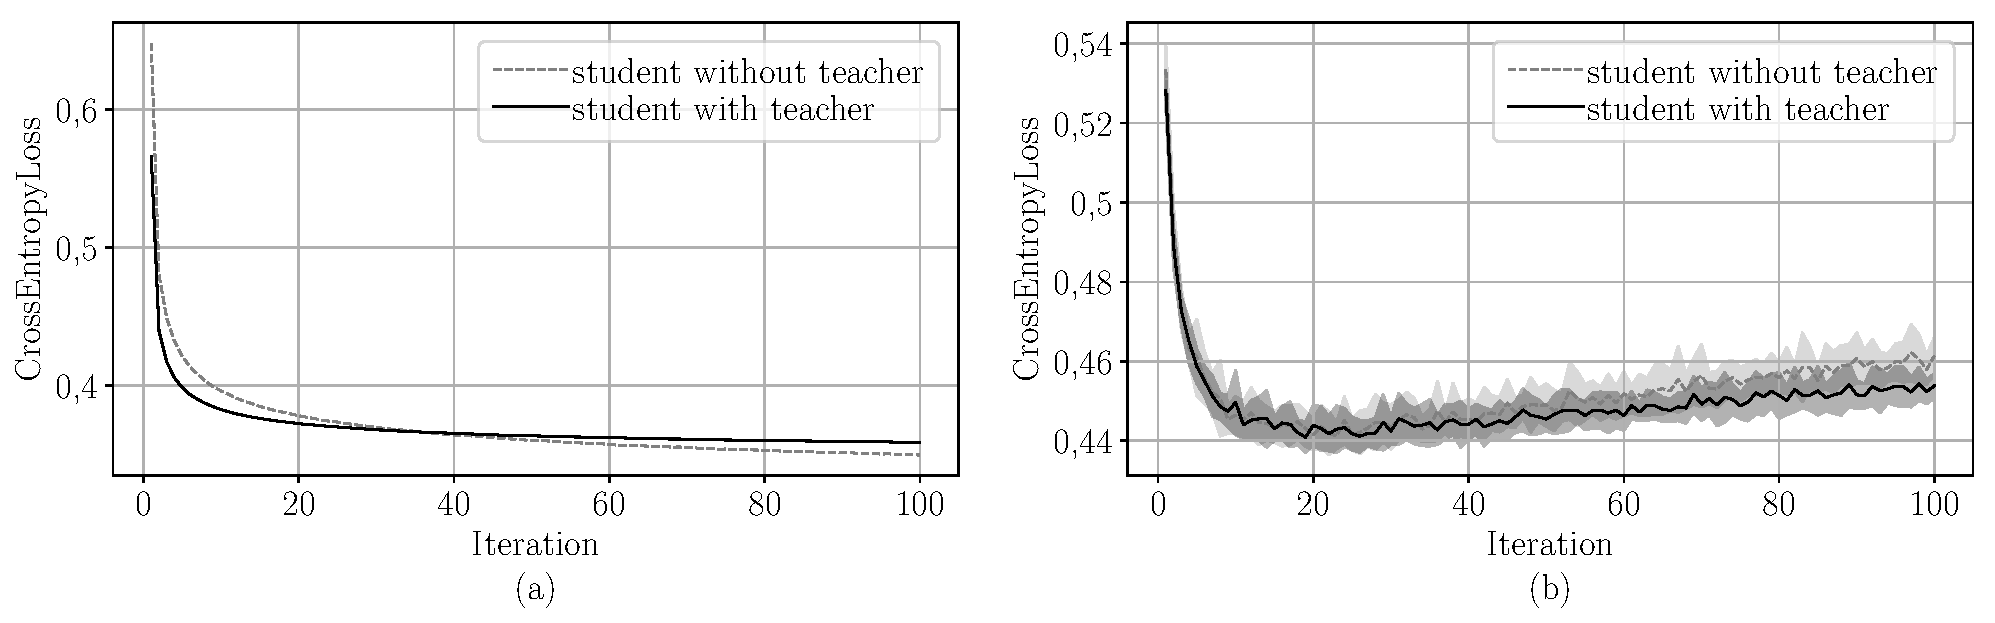
\includegraphics[width=1\textwidth]{results/privlearn/mnist_loss}
\caption{Зависимость кросс--этропии между истинными метками и предсказанными учеников вероятностями классов: a) на обучающей выборке; b) на тестовой выборке}
\label{fg:ex:fashionmnist:loss}
\end{figure}

На рис. \ref{fg:ex:fashionmnist:loss} показан график зависимости кросс--энтропии между истинными метками объектов и вероятностями предсказанными модель ученика. На графике сравнивается модель, которая обучалась без учителя (в задаче оптимизации \eqref{eq:st:class:1} присутствует только первое слагаемое) с моделью полученной путем дистилляции модели нейросети в линейную модель. На графике видно, что обе модели начинают переобучатся после $30-$й итерации, но модель, которая получена путем дистилляции переобувается не так быстро, что следует из того, что ошибка на тестовой выборке растет медленней, а на обучающей выборке падает также медленней.


\paragraph{Синтетический эксперимент.} Проанализируем модель на синтетической выборке. Гипотеза порождения данных:
\begin{gather}
\begin{aligned}
\mathbf{W} &= \left[\mathcal{N}\bigr(w_{jk}|0, 1\bigr)\right]_{n\times K}, \quad &\mathbf{X} &= \left[\mathcal{N}\bigr(x_{ij}|0, 1\bigr)\right]_{m\times n}, \\
 \mathbf{S} &= \text{softmax}\left(\mathbf{XW}\right), \quad &\mathbf{y} &= \left[\text{Cat}\bigr(y_i| \mathbf{s}_i\bigr)\right],
\end{aligned}
\end{gather}
где функция~$\text{softmax}$ берется построчно. Строки матрицы~$\mathbf{S}$ рассматриваются как предсказание учителя, т.е. учитель знает истинные вероятности каждого класса. На рис.~\ref{fg:ex:synt:plate} показана вероятностная модель в графовой нотации. В эксперименте число признаков~$n=10$, число классов~$K=3$, для обучения сгенерировано~$m_{\text{train}}=1000$ и~$m_{\text{test}}=100$ объектов.

На рис.~\ref{fg:ex:synt:distr:real} показано распределение по классам для~$20$ объектов из обучающей выборки. Каждому столбцу на графике соответствует объект, а каждой строке соответствует вероятность класса. Видно, что для каждого рассмотренного объекта вероятности разных классов близки. Получается, что если в качестве истинных меток взять класс с максимальной вероятностью, то выборка будет сильно зашумленной и модель будет описывать эти данные некорректно.

Построим в качестве ученика линейную модель, которая минимизирует кросс-энтропийную (первое слагаемое в формуле~\eqref{eq:st:class:1}). Представление данной модели в виде графовой модели показано на рис.~\ref{fg:ex:synt:plate}.

\begin{figure}[h!t]\center
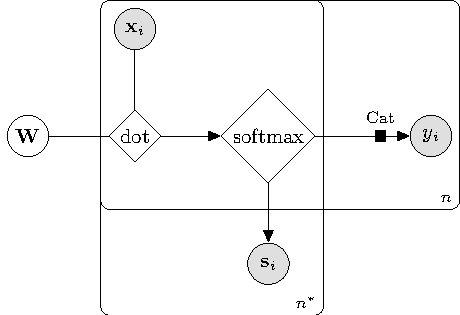
\includegraphics[width=0.35\textwidth]{results/privlearn/linear_model}
\caption{Вероятностная модель используемая в синтетическом эксперименте}
\label{fg:ex:synt:plate}
\end{figure}

\begin{figure}[h!t]\center
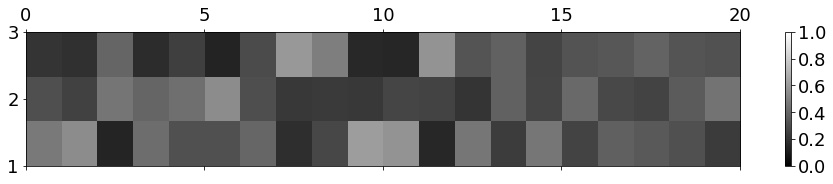
\includegraphics[width=1\textwidth]{results/privlearn/syn_real_distr}
\caption{Истинное распределение  объектов по классам}
\label{fg:ex:synt:distr:real}
\end{figure}


На рис.~\ref{fg:ex:synt:distr:without} показано распределение вероятностей классов, которое предсказала модель. Видно, что полученное распределение не соответствует истинному, так как модель сосредотачивает всю вероятность в одном классе.

\begin{figure}[h!t]\center
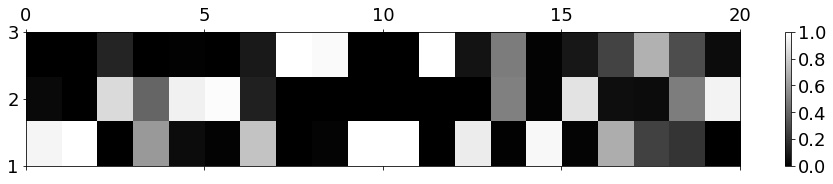
\includegraphics[width=1\textwidth]{results/privlearn/syn_without_teacher_distr}
\caption{Распределение предсказанное моделью без использования информации об истинном распределение на классах}
\label{fg:ex:synt:distr:without}
\end{figure}

\begin{figure}[h!t]\center
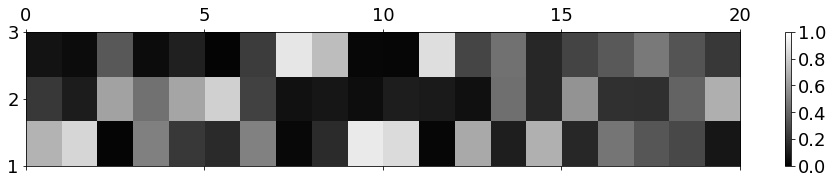
\includegraphics[width=1\textwidth]{results/privlearn/syn_with_teacher_distr}
\caption{Распределение предсказанное моделью c использования информации об истинном распределение на классах}
\label{fg:ex:synt:distr:with}
\end{figure}

\begin{figure}[h!t]\center
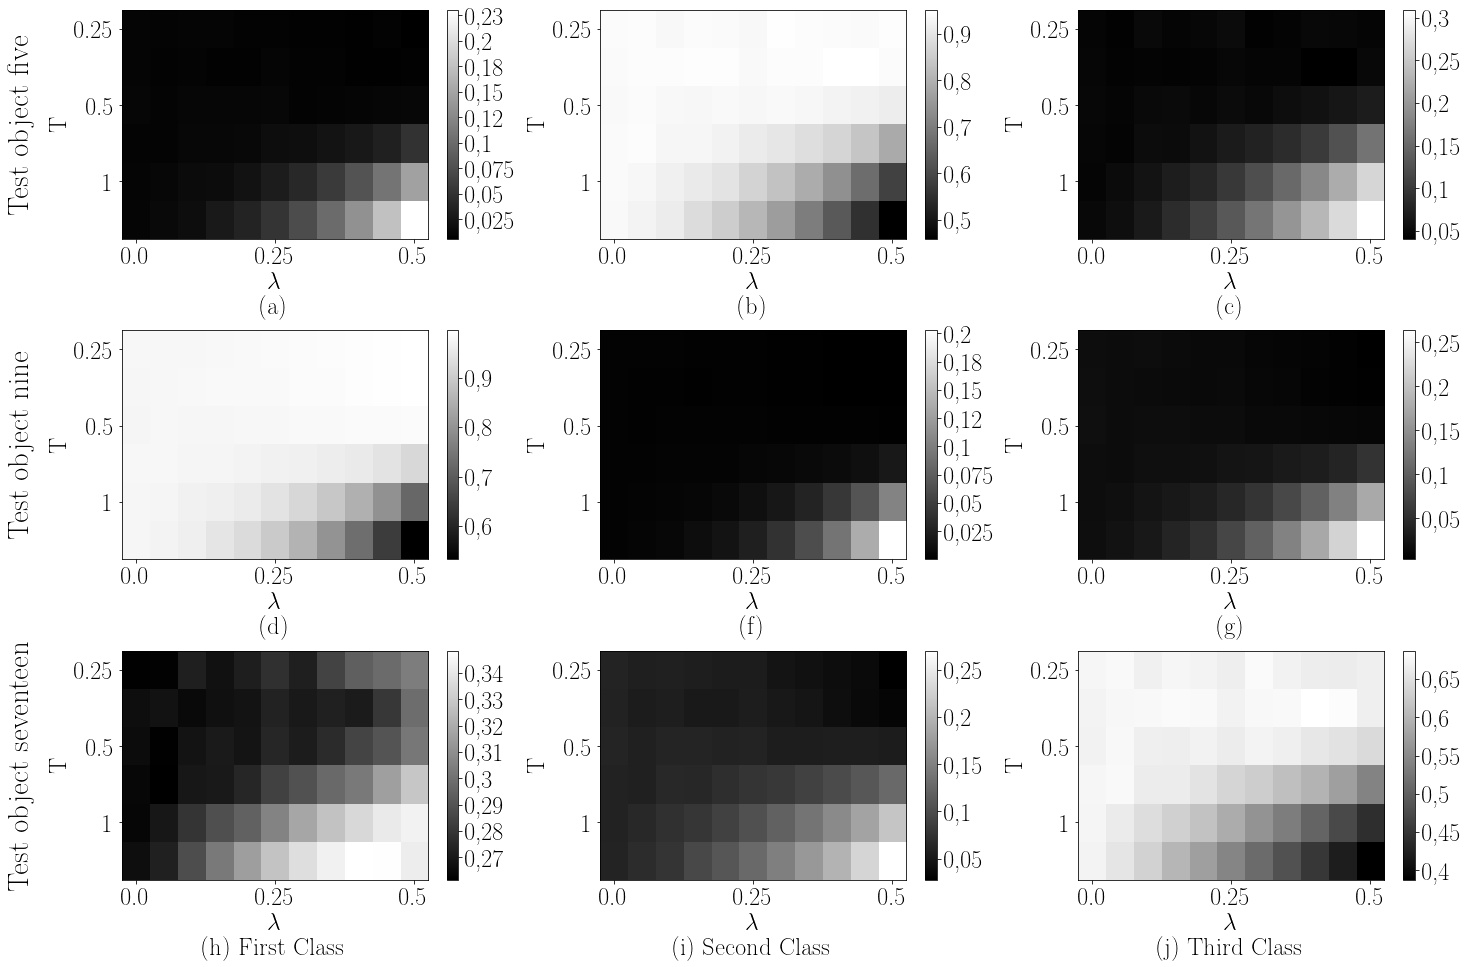
\includegraphics[width=1\textwidth]{results/privlearn/syn_T_lambda}
\caption{Вероятности классов для разных объектов}
\label{fg:ex:synt:distr:lambda_T}
\end{figure}

Рассмотрим модель, которая учитывает информацию об истинных распределениях на классах для каждого объекта. Для этого минимизируются первые три слагаемых в формуле~\eqref{eq:st:class:1} при~$T_0=1$ и~$\lambda=0{,}75$. В качестве меток учителя~$s_{i,k}$ использовались истинные вероятности для каждого класса данного объекта. На рис.~\ref{fg:ex:synt:distr:with} показано распределение, которое дала модель. В данном случае видно, что распределения являются сглаженными. Концентрации всей вероятности в одном классе не наблюдается.

Заметим, что в данном примере предполагается, что модель учителя учитывает не только метки классов, но и распределение на метках классов, в то время как в выборке~$\{\mathbf{X}, \mathbf{y}\}$ имеются только точечные оценки в виде меток. 

В данном примере используются истинные распределения в качестве предсказаний учителя, но их можно заменить предсказаниями модели учителя, которая предсказывает не только сами метки, но и их распределение для каждого объекта.

На рис.~\ref{fg:ex:synt:distr:lambda_T} показана зависимость вероятности верного класса от температуры~$T$ и параметра доверия~$\lambda$ для одного из объектов из тестовой выборки. На рис.~\ref{fg:ex:synt:distr:lambda_T} видно, что изменение температуры~$T$ влечет изменение концентрации вероятностной меры. При уменьшении параметра температуры и приближении его к нулю наблюдаем, что вероятность одного из классов приближается к единице, а остальных классов~--- к нулю. С другой стороны, при увеличении параметра температуры вероятности классов сглаживаются и распределение классов для каждого объекта становится близким к равномерному.

В таблице~\ref{tb:ce:1} в колонке ``Кросс-энтропийная ошибка с реальными вероятностями'' показано сравнение кросс-энтропии в случае, если в качестве истинных вероятностей меток рассмотреть не onehot-кодированные вероятности классов, а истинные вероятности:
\begin{gather}
\label{eq:ce:1}
\begin{aligned}
\mathcal{L}_{\text{real}}\bigr(\mathbf{g}\bigr) = - \sum_{i=1}^{m}\sum_{k=1}^{K}s_{i}^{k}\log g_k\bigr(\mathbf{x}_i\bigr),
\end{aligned}
\end{gather}
где~$\mathbf{g}$~--- модель ученика. Видно, что модель с учителем лучше аппроксимирует истинные вероятности классов. Также в таблице~\ref{tb:ce:1}
представлено среднее значение разницы максимальной вероятности с минимальной вероятностью для каждого объекта:
\begin{gather}
\label{eq:ce:2}
\begin{aligned}
\mathcal{L}_{\text{maxmin}}\bigr(\mathbf{g}\bigr) = \frac{1}{m}\sum_{i=1}^{m}\left(\max_{k}g_k\bigr(\mathbf{x}_i\bigr) -  \min_{k}g_k\bigr(\mathbf{x}_i\bigr)\right).
\end{aligned}
\end{gather}
Видно, что модель учителя имеет меньшую разницу между вероятностями классов, т.е. вероятности классов не концентрируются в одном классе.


\paragraph{Анализ твитов пользователей.}Проводится эксперимент на выборке Twitter Sentiment Analysis. Данная выборка содержит короткие сообщения, для которых требуется предсказать эмоциональный окрас: содержит твит позитивный окрас или негативный. Выборка разделена на~$1{,}18$ млн твитов для обучения и~$0{,}35$ млн твитов для тестирования. Выполнена предобработка твитов: все твиты переведены в нижний регистр, все никнеймы вида~``@andrey'' заменены на токен ``name'', все цифры заменены на токен ``number''.

Результаты данной части эксперимента показаны в таблице. В качестве модели учителя использовалась модель Bi-LSTM с линейным слоем на выходе. В качестве векторного представления токенов обучалась матрица параметров. В ней каждая строка соответствует токену из обучающей выборки. Суммарное число обучаемых параметров модели учителя составляет более~$30$ млн. Обученная модель учителя имеет точность предсказания~$0{,}835$. В качестве модели ученика рассматривается линейная модель с $1538$ параметрами, где в качестве векторного представления предложения рассматривается выход предобученной модели BERT с размерностью векторного пространства~$768$. Признаковое описание модели учителя и модели ученика различаются. Модель учителя в качестве признакового описания рассматривает исходные слова в предложении. Модель ученика в качестве признакового описания использует готовое векторное представление предложения, которое получено при помощи модели BERT.

В таблице~\ref{tb:ce:1} показано качество модели ученика с использованием предсказания модели учителя и без него. В рамках данных результатов качество модели ученика с дистилляцией выше, чем модели ученика без дистилляции, но разница находится в пределах погрешности, что не позволяет говорить о значительных улучшениях качества.

\begin{table}[]
\caption{Сводная таблица результатов вычислительного эксперимента}
\label{tb:ce:1}
\begin{center}
\resizebox{\textwidth}{!}{
\begin{tabular}{|l|c|c|c|c|c|c|}
\hline
\multicolumn{1}{|c|}{Выборка} & Модель      & \begin{tabular}[c]{@{}c@{}}Кросс-Энтропийная\\ ошибка\end{tabular} & \begin{tabular}[c]{@{}c@{}}Кросс-Энтропийная \\ ошибка с реальными\\ вероятностями\end{tabular} & \begin{tabular}[c]{@{}c@{}}Вероятностная\\ разница\end{tabular} & Точность            & \begin{tabular}[c]{@{}c@{}}Число\\ Параметров\end{tabular} \\ \hline\hline
\multirow{2}{*}{FashionMnist} & с учителем  & $0{,}453\pm0{,}003$                                                & -                                                                                             & $0{,}84\pm0{,}13$                                               & $0{,}842\pm0{,}002$ & 7850                                                       \\ \cline{2-7} 
                              & без учителя & $0{,}461\pm0{,}005$                                                & -                                                                                             & $0{,}86\pm0{,}18$                                               & $0{,}841\pm0{,}002$ & 7850                                                       \\ \hline \hline
\multirow{2}{*}{Systetic}     & с учителем  & $0{,}618\pm0{,}001$                                                & $1{,}17\pm0{,}05$                                                                             & $0{,}45\pm0{,}20$                                               & $0{,}828\pm0{,}002$ & 33                                                         \\ \cline{2-7} 
                              & без учителя & $0{,}422\pm0{,}002$                                                & $2{,}64\pm0{,}02$                                                                             & $0{,}75\pm0{,}22$                                               & $0{,}831\pm0{,}001$ & 33                                                         \\ \hline \hline
\multirow{2}{*}{Twiter}       & с учителем  & $0{,}489\pm0{,}003$                                               & -                                                                                             & $0{,}79\pm0{,}17$                                               & $0{,}764\pm0{,}005$ & 1538                                                       \\ \cline{2-7} 
                              & без учителя &  $0{,}501\pm0{,}006$                                                & -                                                                                             & $0{,}83\pm0{,}22$                                               & $0{,}747\pm0{,}004$ & 1538                                                       \\ \hline 
\end{tabular}
}
\end{center}
\end{table}

В таблице~\ref{tb:ce:1} 
показаны результаты вычислительного эксперимента для разных выборок. Из результатов эксперимента видно, что модель ученика наследует распределение вероятностей по классам от модели учителя. Когда модель учителя адекватно описывает данные, то описание данных моделью ученика также улучшается, что показано в вычислительном эксперименте на синтетических данных. Показано, что точность аппроксимации выборки учеником повышается при использовании модели учителя. Задача регрессии не приведена в вычислительном эксперименте, так как в теореме~\ref{theorem:st:reg} показана ее эквивалентность задаче линейной регрессии. Для задачи классификации проведен вычислительный эксперимент. Из вычислительного эксперимента видно, что дистилляция влияет на распределение классов в рамках одного объекта. Вероятности классов для каждого объекта являются более разреженными, а не концентрируются в одном классе. Данное свойство хорошо видно в синтетической выборке, так как она генерировалась с максимальной дисперсией в вероятностях классов.